\documentclass{article}
\usepackage{graphicx} % Required for inserting images
\usepackage{lipsum} % For dummy text
\usepackage{xcolor}
% Adjust margins
\usepackage{geometry}
\geometry{margin=2cm}

\title{\textbf{Entomological digital evidence to estimate time since death in forensic investigations}}
\author{Dr. Charansing N. Kayte}
\date{13 May 2024}

\begin{document}
\maketitle

\begin{abstract}
In this research, the focus is on creating the image database of forensically significant insects, and further, the images have been collected using python software to collect image features. This database can be used by certain smartphone apps that will assess the criminal investigation of the death time of the dead body. The results will be produced within a limited time so the enforcement agencies such as police investigating team need not wait for the post mortem and forensic lab reports to estimate the time elapsed since death.\\
Keyword: Python, Autolysis, Skeletenization, Cadaver, ImageJ
\end{abstract}

\section*{1. INTRODUCTION}
Forensic investigations include one important aspect of the use of insects and other arthropods in the estimation of time since death, this is known as forensic entomology. The decomposition of the body is been divided into 4 stages, which include 

\subsection*{1.1. Autolysis}
Autolysis is self-digestion, and it starts right after death. The cessation of blood circulation and respiration results in the rupture of the cell membrane and ultimately the skin starts loosening from the body. 
\subsection*{1.2. Bloat}
The second stage is of bloating where the gases filled in the body make it swollen. 
\subsection*{1.3. Active Decay}
The third stage starts as the fluids start releasing from the body resulting in active decay of the body.
\subsection*{1.4. Skeletenization}
At the end of the decomposition, the body gets skeletonized with the only remains of bones of cadaver.\\
Insects arrive in a specific order at a decomposing organism and then complete their life cycle depending on the temperature around it. We also observed the life cycle of insects in the closed house and outside the home for all three seasons (summer, monsoon, and winter).

\begin{figure}[ht]
    \centering
    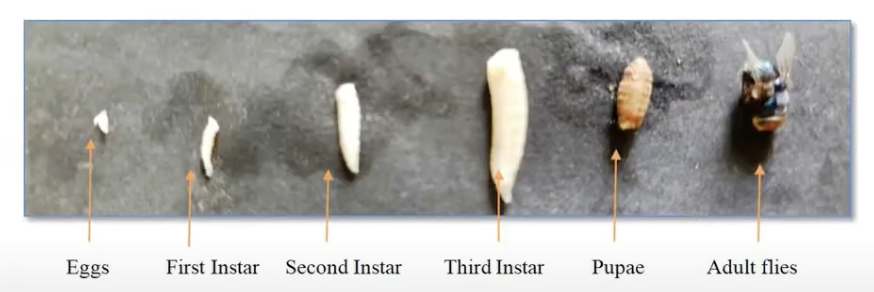
\includegraphics[width=0.8\textwidth]{fig01.png}
    \caption{Different Stages of Insect Life Cycle}
    \label{fig:insect-life-cycle}
\end{figure}

As shown in Figure~\ref{fig:insect-life-cycle}, the different stages of the insect life cycle are crucial in estimating the time since death.

\section*{2. EXPERIMENTAL METHOD}
\subsection*{2.1. Sample collection}
Samples of insects of all stages be collected from different areas of the body (sample body of dead goat), from the clothing and the soil. In between research we have capture photo images with reference objects of every stage of the insect life cycle and preserved collected samples of all stages. After that, we have been calculating the size of the insect-based on season and temperature.
\subsection*{2.2. Collection of stages}
Once the sample was kept, the constant observation was done at a particular time, particularly three times a day (10 am, 2 pm, and 5 pm). Once we observed any stage on the sample it was collected with help of rubber-tipped forceps and a soft brush and kept in a dry airtight container. For collecting the adult fly we used a standard net.
\subsection*{2.3. Sample preservation}
The eggs were preserved in 70\% ethanol, instar stages were preserved in KAA (kerosene, acetic acid, and ethyl alcohol) solution. We preserve pupae in an airtight bottle. For the adult flies after killing, we used an airtight bottle with a cotton base for sample preservation.

\end{document}
